\documentclass[12pt,a4paper]{article}
\usepackage[utf8]{inputenc}
\usepackage{amsfonts}
\usepackage{amssymb}
\usepackage{graphicx}
\usepackage{float}

% sets margin
\usepackage[hmargin=3cm,vmargin=2.5cm]{geometry}

% creates landscape pages
\usepackage{pdflscape}
\usepackage{pdfpages}

%\renewcommand{\rmdefault}{phv} % Arial
\renewcommand{\sfdefault}{phv} % Arial

% defining settings for textpos
\usepackage[absolute]{textpos}
\setlength{\TPHorizModule}{\paperwidth}
\setlength{\TPVertModule}{\paperheight}

% headers / footers
\usepackage{fancyhdr}
\pagestyle{fancy}
\fancyhf{}
\rhead{Assignment 2}
\lhead{CSP2348: Data Structures}
\rfoot{\thepage}
\lfoot{Martin Ponce, ID: 10371381}
\renewcommand{\footrulewidth}{0.5pt}

% defining landscape headers / footers
\fancypagestyle{fancylscape}{
	\fancyhf{}
	\renewcommand{\footrulewidth}{0pt}
	\renewcommand{\headrulewidth}{0pt}
	% header
	\begin{textblock}{0.05}[-0.5,-2](0,0)
		{\rotatebox{90}{CSP2348: Data Structures}}
	\end{textblock}
		\begin{textblock}{0.05}[-0.5,-1](0,0)
		{\rotatebox{90}{Assignment 2}}
	\end{textblock}
	\begin{textblock}{0.05}[-1,-0.109](0,0)
		{\rotatebox{90}{\rule{24.2cm}{0.5pt}}}
	\end{textblock}
	% footer
	\begin{textblock}{0.05}[-19,-4.28](0,0)
		{\rotatebox{90}{Martin Ponce, ID: 10371381}}
	\end{textblock}
		\begin{textblock}{0.05}[-19,-12.8](0,0)
		{\rotatebox{90}{\thepage}}
	\end{textblock}
		\begin{textblock}{0.05}[-18.7,-0.109](0,0)
		{\rotatebox{90}{\rule{24.2cm}{0.5pt}}}
	\end{textblock}
}

% adjusts padding between caption and figure
\setlength{\belowcaptionskip}{10pt}

% adds links to references and colors them blue
\usepackage{hyperref}
\hypersetup{colorlinks=true,
			linkcolor=blue,
			citecolor=black,
			urlcolor=blue}

% apa style referencing
\usepackage[sectionbib, natbibapa]{apacite}
\usepackage{chbibref}

% underlining text
\usepackage[normalem]{ulem}

% \citetapos for possesive citations
\newcommand{\citetapos}[1]{\citeauthor{#1}{\textcolor{black}{'s}} \citeyearpar{#1}}

% add multiline comments \begin{comment} \end{comment}
\usepackage{verbatim}

% add minted package for code highlighting
\usepackage[section]{minted}

\usepackage{tcolorbox}
\tcbuselibrary{minted,skins}

\newtcblisting{javacode}{
  listing engine=minted,
  colback=bg,
  colframe=black!70,
  listing only,
  minted style=monokai,
  minted language=java,
  minted options={linenos=true,texcl=true},
  left=1mm,
}
\definecolor{bg}{rgb}{0.20,0.20,0.20}

% front matter
\title{Edith Cowan University\\CSP2348\\Data Structures\\Assignment 2}
\author{Martin Ponce\\Student 10371381\\\\Tutor: Jitian Xiao}
\date{\today}

\begin{document}

% title page
\newpage
\null  % Empty line
\nointerlineskip  % No skip for prev line
\vfill
\let\snewpage \newpage
\let\newpage \relax
\maketitle
\thispagestyle{empty}
\let \newpage \snewpage
\vfill

% toc
\newpage
\tableofcontents
\thispagestyle{fancy}

\newpage
\section{Introduction}

The Board of Directors at Blue Ink have recently become aware of the lack of computer security awareness and best practices amongst its employees. As a result, Blue Ink have requested that a sample Virtual Machine (VM) image of a typical computer within their organisation be analysed for security issues.

This report outlines the security issues identified during the analysis of Blue Ink's sample VM image. Vulnerabilities have been found with the operating system itself, and support software packaged with the operating system, such as the Internet browser and anti-virus application. Vulnerabilities have also been identified in outdated software whilst practices regarding the storage of passwords in plain-text files within user documents folders provide opportunities for unwanted access. The security issues identified in this report must be addressed in order to maintain the utmost security.

\subsection{Assumptions}

\begin{itemize}
\item A firewall is implemented within the network
\end{itemize}

%\newpage
\section{Task 2: Advanced normalisation}

Figure 2 below depicts an invoice for an order from a store.

\begin{figure}[H]
\centering
\caption{Pakoko Tax Invoice}
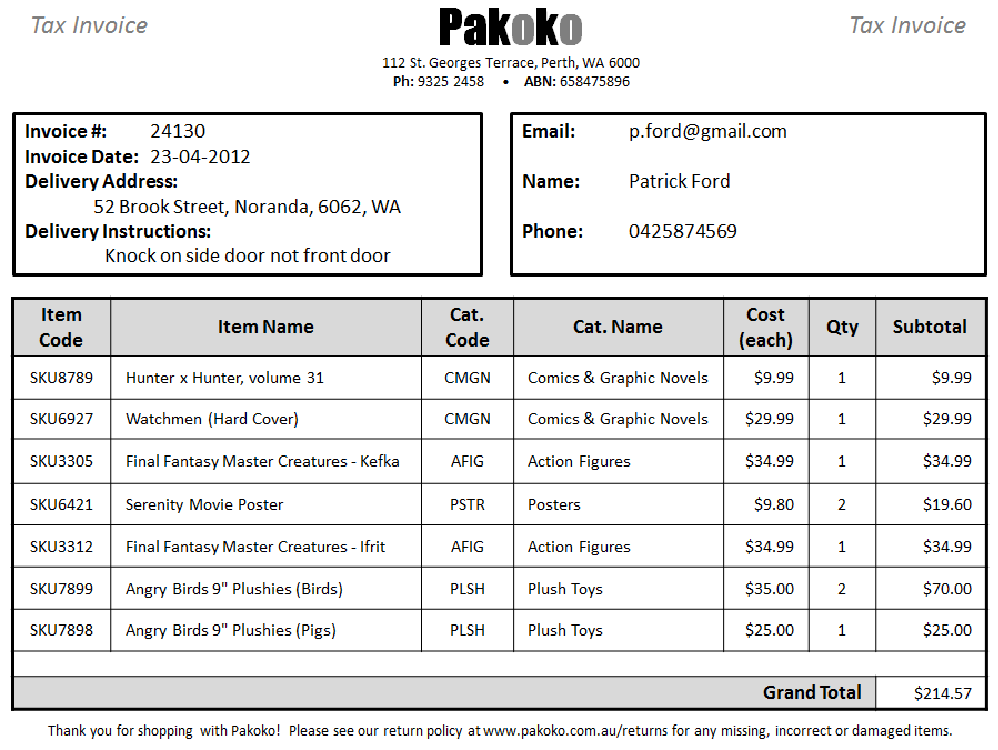
\includegraphics[scale=0.75]{./img/task2.pdf}
\end{figure}

\subsection*{Assumptions}

\begin{itemize}
\item Auto-incrementing Cust\# has been created, replacing CustEmail as customer identifier
	\begin{itemize}
	\item Auto-incrementing identifier avoids user input error which may result in multiple customers with the same email address
	\item Allows CustEmail to be updated without having to update foreign keys if CustEmail remained as identifier
	\end{itemize}
\item Each item is only in one category
\item Item codes are unique per item, even if the items are in different categories
\item Invoice header and footer is static and is not stored in the database
	\begin{itemize}
	\item Includes Pakoko business details header and thank you / return policy URL footer
	\end{itemize}
\item Derived attributes are not stored in the database
	\begin{itemize}
	\item Includes Item Subtotal and Invoice Grand Total
	\end{itemize}
\end{itemize}

\subsection{0NF: Unnormalised form}

R1 = (Cust\#, CustEmail, CustName, CustPhone, DeliveryAddress, DeliveryInstructions, \{Invoice\#, InvoiceDate, \{ItemCode, ItemName, CatCode, CatName, Cost, Qty\}\})

\subsection{1NF: First normal form}

\sout{R1 = (\textbf{\underline{Cust\#}}, CustEmail, CustName, CustPhone, DeliveryAddress, DeliveryInstructions, \{\textbf{\underline{Invoice\#}}, InvoiceDate, \{\textbf{\underline{ItemCode}}, ItemName, CatCode, CatName, Cost, Qty\}\})}
\\\\
R11 = (\textbf{\underline{Cust\#}}, CustEmail, CustName, CustPhone, DeliveryAddress, DeliveryInstructions)
\\\\
R12 = (\textbf{\underline{Invoice\#}}, InvoiceDate, \emph{Cust\#})
\\\\
R13 = (\textbf{\underline{\emph{Invoice\#}}}, \textbf{\underline{ItemCode}}, ItemName, CatCode, CatName, Cost, Qty)

\subsection{2NF: Second normal form}

R11 = (\textbf{\underline{Cust\#}}, CustEmail, CustName, CustPhone, DeliveryAddress, DeliveryInstructions)
\\\\
R12 = (\textbf{\underline{Invoice\#}}, InvoiceDate, \emph{Cust\#})
\\\\
\sout{R13 = (\textbf{\underline{\emph{Invoice\#}}}, \textbf{\underline{ItemCode}}, ItemName, CatCode, CatName, Cost, Qty)}
\\\\
R131 = (\textbf{\underline{\emph{Invoice\#}}}, \textbf{\underline{\emph{ItemCode}}}, Qty)
\\\\
R132 = (\textbf{\underline{ItemCode}}, ItemName, CatCode, CatName, Cost)

\subsection{3NF: Third normal form}

R11 = (\textbf{\underline{Cust\#}}, CustEmail, CustName, CustPhone, DeliveryAddress, DeliveryInstructions)
\\\\
R12 = (\textbf{\underline{Invoice\#}}, InvoiceDate, \emph{Cust\#})
\\\\
R131 = (\textbf{\underline{\emph{Invoice\#}}}, \textbf{\underline{\emph{ItemCode}}}, Qty)
\\\\
\sout{R132 = (\textbf{\underline{ItemCode}}, ItemName, CatCode, CatName, Cost)}
\\\\
R1321 = (\textbf{\underline{ItemCode}}, ItemName, \emph{CatCode})
\\\\
R1322 = (\textbf{\underline{CatCode}}, CatName)

\subsection{Named relations}

Customer = (\textbf{\underline{Cust\#}}, CustEmail, CustName, CustPhone, DeliveryAddress, DeliveryInstructions)
\\\\
Invoice = (\textbf{\underline{Invoice\#}}, InvoiceDate, \emph{Cust\#})
\\\\
InvoiceItem = (\textbf{\underline{\emph{Invoice\#}}}, \textbf{\underline{\emph{ItemCode}}}, Qty)
\\\\
Item = (\textbf{\underline{ItemCode}}, ItemName, \emph{CatCode})
\\\\
Category = (\textbf{\underline{CatCode}}, CatName)

\subsection{Physical E-R diagram}
%\section{Task 3: Entity-Relationship modelling}

\subsection{Logical E-R diagram}

\subsection{Physical E-R diagram}
%\section{Task 4: Advanced Entity-Relationship modelling}

\subsection{Logical E-R diagram}

\subsection{Physical E-R diagram}

\newpage
\urlstyle{rm}
%\setbibref{\textsf{References}}
\bibliographystyle{apacite}
\addcontentsline{toc}{section}{References}
%\bibliography{./bib/Year 1-Sem 2-CSI1101-A1}

\end{document}